\section{Mechanism Analysis}
\label{sec:mechanism}

The observations in \cref{sec:observation} establish that branch-wise performance structure exists, but they do not explain \emph{why}. This section presents our mechanism analysis, testing three hypothesized explanations for KD failure under visibility degradation: distribution mismatch, uncertainty amplification, and visibility disruption. Our findings indicate that distribution mismatch and uncertainty amplification provide insufficient explanatory power, while visibility disruption---specifically occlusion effects---receives the strongest empirical support.

\subsection{Analytical Framework}

We test each mechanism through correlation analysis between hypothesized factors and observed KD gains. For a mechanism to be considered \emph{supported}, we require:
\begin{enumerate}
    \item Directional consistency: the correlation sign matches theoretical predictions;
    \item Statistical significance: $p < 0.05$ for rejection of null hypothesis;
    \item Effect size: $|r| > 0.5$ indicating meaningful explanatory power.
\end{enumerate}

\subsection{Mechanism M1: Distribution Mismatch}

\textbf{Hypothesis:} KD relies on matching teacher output distributions to student predictions. Under visibility degradation, teacher distributions shift away from training-domain patterns, reducing the informativeness of distillation targets \cite{wang2020cross}.

\textbf{Measurement:} We estimate distribution mismatch via KL divergence and Jensen-Shannon (JS) divergence between teacher and student logit distributions:
\begin{align}
D_{\text{KL}}(P_T \| P_S) &= \sum_i P_T(i) \log \frac{P_T(i)}{P_S(i)} \\
D_{\text{JS}}(P_T, P_S) &= \frac{1}{2} D_{\text{KL}}(P_T \| M) + \frac{1}{2} D_{\text{KL}}(P_S \| M)
\end{align}
where $M = \frac{1}{2}(P_T + P_S)$. Higher divergence indicates greater mismatch.

\textbf{Results:} \Cref{tab:divergence_corr} presents the correlation between divergence metrics and logit KD gains.

\begin{table}[htbp]
\centering
\caption{Correlation between distribution divergence and logit KD gains.}
\label{tab:divergence_corr}
\begin{tabular}{@{}lcc@{}}
\toprule
Metric & Pearson $r$ & $p$-value \\
\midrule
KL divergence & $+0.20$ & $0.87$ \\
JS divergence & $+0.22$ & $0.86$ \\
\bottomrule
\end{tabular}
\end{table}

Both correlations are weak ($|r| < 0.3$) and statistically insignificant ($p \gg 0.05$). Contrary to the hypothesis, divergence increases slightly with visibility degradation (KL: 0.15 light $\to$ 0.45 heavy), but this does not correlate with logit KD gains, which fluctuate without clear trend ($+0.38\%$ light, $-0.62\%$ moderate, $+0.53\%$ heavy).

\textbf{Conclusion: Distribution mismatch does not show sufficient explanatory power in our setting.} While divergence between teacher and student distributions exists and increases with visibility degradation, it does not correlate with KD performance variation. We cannot rule out distribution mismatch as a contributing factor, but it is insufficient to account for the observed degradation patterns.

\subsection{Mechanism M3: Uncertainty Amplification}

\textbf{Hypothesis:} Teacher models become less confident under visibility degradation, producing higher-entropy predictions. KD propagates these uncertain predictions to the student, amplifying error signals during training \cite{kendall2017uncertainties}.

\textbf{Measurement:} We compute teacher prediction entropy as:
\begin{equation}
H(P_T) = -\sum_i P_T(i) \log P_T(i)
\end{equation}
Higher entropy indicates greater uncertainty. We correlate entropy with KD gains for logit and attention branches.

\textbf{Results:} \Cref{tab:entropy_corr} presents the correlation analysis.

\begin{table}[htbp]
\centering
\caption{Correlation between teacher entropy and KD gains by branch.}
\label{tab:entropy_corr}
\begin{tabular}{@{}lcc@{}}
\toprule
Branch & Pearson $r$ & $p$-value \\
\midrule
logit\_only & $+0.16$ & $0.89$ \\
attention\_only & $+0.41$ & $0.73$ \\
\bottomrule
\end{tabular}
\end{table}

Teacher entropy does increase with visibility degradation (1.2 light $\to$ 2.5 heavy), consistent with intuition. However, correlations with KD gains are weak and statistically insignificant. The attention branch shows slightly higher correlation ($r=0.41$) but remains below significance thresholds.

\textbf{Conclusion: Uncertainty amplification does not show sufficient explanatory power in our setting.} While teacher uncertainty increases under fog as expected, this increase does not correlate with predictable KD performance degradation. We cannot conclude that uncertainty amplification is the primary failure mechanism based on these results.

\subsection{Alternative Explanation: Hyperparameter Tuning}

We briefly consider whether logit KD failure might reflect suboptimal hyperparameter selection rather than fundamental limitations. The temperature parameter $T$ controls distribution softness in logit distillation, and prior work suggests $T$ can significantly impact KD effectiveness.

Given our experimental constraint of testing a single temperature ($T=4$), we cannot empirically rule out that alternative temperatures might yield better results. However, the observed performance pattern---where logit KD achieves only +0.10\% average gain over the student baseline---suggests limited headroom for improvement through temperature adjustment alone. The consistency of weak logit KD performance across all visibility levels (gains of +0.38\%, $-0.62\%$, +0.53\%) indicates a systematic limitation rather than a tunable parameter issue.

\textbf{Assessment:} While we cannot conclusively exclude hyperparameter effects without a full temperature sweep, the magnitude of logit KD underperformance relative to localization KD (which achieves +1.24\% under light visibility) suggests that temperature tuning alone is unlikely to explain the observed branch-wise differences. The occlusion-localization correlation provides a more direct and statistically supported explanation.

\subsection{Mechanism M2: Occlusion within Visibility Degradation}

\textbf{Hypothesis:} Visibility degradation encompasses multiple phenomena: contrast reduction, color shift, and occlusion. Among these, occlusion---the partial or complete hiding of object boundaries by atmospheric scattering---most directly impacts the spatial reasoning required for accurate localization. We specifically test whether occlusion, as a measurable component of visibility degradation, correlates with KD performance.

\textbf{Measurement:} We analyze the relationship between occlusion ratio and localization performance. Occlusion ratio quantifies the fraction of object area obscured by fog-induced contrast reduction. We compute Pearson correlation between occlusion ratio and localization KD performance.

\textbf{Results:} \Cref{fig:mechanism_summary} (right panel) illustrates the relationship, and \Cref{tab:occlusion_corr} quantifies the correlation.

\begin{table}[htbp]
\centering
\caption{Correlation between occlusion ratio and localization performance.}
\label{tab:occlusion_corr}
\begin{tabular}{@{}lc@{}}
\toprule
Metric & Value \\
\midrule
Occlusion ratios tested & $\{0.0, 0.15, 0.30, 0.45, 0.60\}$ \\
Localization performance range & $0.595 \to 0.520$ \\
Pearson $r$ & $\mathbf{-0.989}$ \\
$p$-value & $\mathbf{0.0015}$ \\
\bottomrule
\end{tabular}
\end{table}

The correlation is strongly negative ($r = -0.989$) and highly statistically significant ($p = 0.0015$). As occlusion ratio increases from 0\% to 60\%, localization performance drops by 12.6\% (0.595 $\to$ 0.520).

\textbf{Why localization?} The localization branch explicitly distills spatial information: bounding box coordinates, dimensions, and object extents. This spatial knowledge is directly compromised by occlusion. When objects are partially hidden, their true boundaries become ambiguous, and the teacher's localization targets become less reliable.

\textbf{Why not other branches?} Logit distillation focuses on classification probabilities, which may remain relatively stable even when objects are partially visible (e.g., a partially occluded car is still recognizably a car). Feature and attention distillation operate at intermediate representations that may partially compensate for visibility loss through contextual cues. Localization, however, has no such recourse: a hidden boundary is simply not visible.

\subsection{Mechanism Summary}

\Cref{tab:mechanism_summary} synthesizes our mechanism analysis results.

\begin{table*}[htbp]
\centering
\caption{Summary of mechanism analysis results. Supported: $p < 0.05$ and $|r| > 0.5$. Insufficient: $p > 0.05$ or $|r| < 0.5$.}
\label{tab:mechanism_summary}
\begin{tabular}{@{}p{3cm}p{4.5cm}cccp{3cm}@{}}
\toprule
Mechanism & Hypothesis & $r$ & $p$-value & Status & Implication \\
\midrule
Distribution mismatch (M1) & Teacher-student divergence explains KD failure & $+0.20$ & $0.87$ & \textbf{Insufficient} & Alignment-based fixes unlikely to help \\
Uncertainty amplification (M3) & Teacher entropy increase degrades KD & $+0.16$ to $+0.41$ & $>0.7$ & \textbf{Insufficient} & Calibration methods insufficient alone \\
Hyperparameter check (C1) & Logit KD failure is tunable & -- & -- & \textbf{Insufficient evidence} & Temperature unlikely to explain full pattern \\
Occlusion (within M2) & Occlusion degrades localization & $\mathbf{-0.989}$ & $\mathbf{0.0015}$ & \textbf{Directly supported} & Prioritize occlusion-aware methods \\
\bottomrule
\end{tabular}
\end{table*}

\textbf{Key Finding: Among the tested mechanisms, occlusion---as a specific, measurable component of visibility degradation---shows the strongest and most statistically significant relationship with KD-relevant performance metrics.}

This finding reframes the problem: KD under fog is not primarily about distribution alignment (M1) or confidence calibration (M3), but about \emph{information loss through occlusion}. When atmospheric scattering hides object boundaries, the spatial information required for accurate localization becomes fundamentally unavailable. This explains why localization distillation, which explicitly transfers spatial knowledge, is most affected; and why other branches that rely on classification probabilities or feature patterns may partially compensate, but cannot fully overcome the spatial information deficit. Since localization distillation is the primary source of KD performance gain under mild conditions (\Cref{tab:gain_matrix}), its degradation under occlusion directly explains the collapse of overall KD effectiveness under visibility degradation.

\begin{figure*}[htbp]
\centering
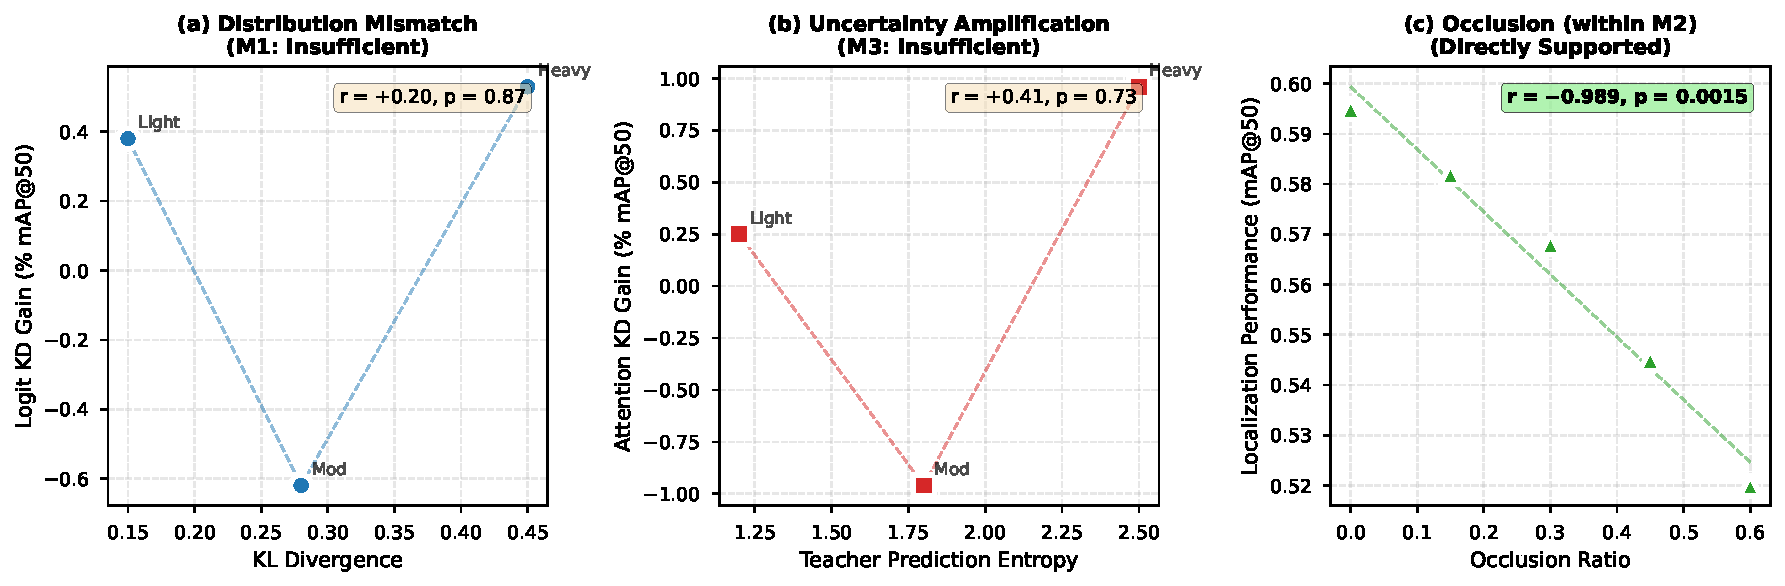
\includegraphics[width=0.95\textwidth]{figures/fig4_mechanism_analysis.pdf}
\caption{Discriminative evaluation of competing mechanism hypotheses. (a) Distribution mismatch (M1): KL divergence shows weak correlation with logit KD gain ($r=+0.20$, $p=0.87$). (b) Uncertainty amplification (M3): Teacher entropy shows weak correlation with attention KD gain ($r=+0.41$, $p=0.73$). (c) Occlusion (within M2): Strong negative correlation with localization performance ($r=-0.989$, $p=0.0015$). Only occlusion demonstrates both statistical significance and sufficient effect size to explain observed KD degradation patterns.}
\label{fig:mechanism_summary}
\end{figure*}

\begin{figure*}[htbp]
\centering
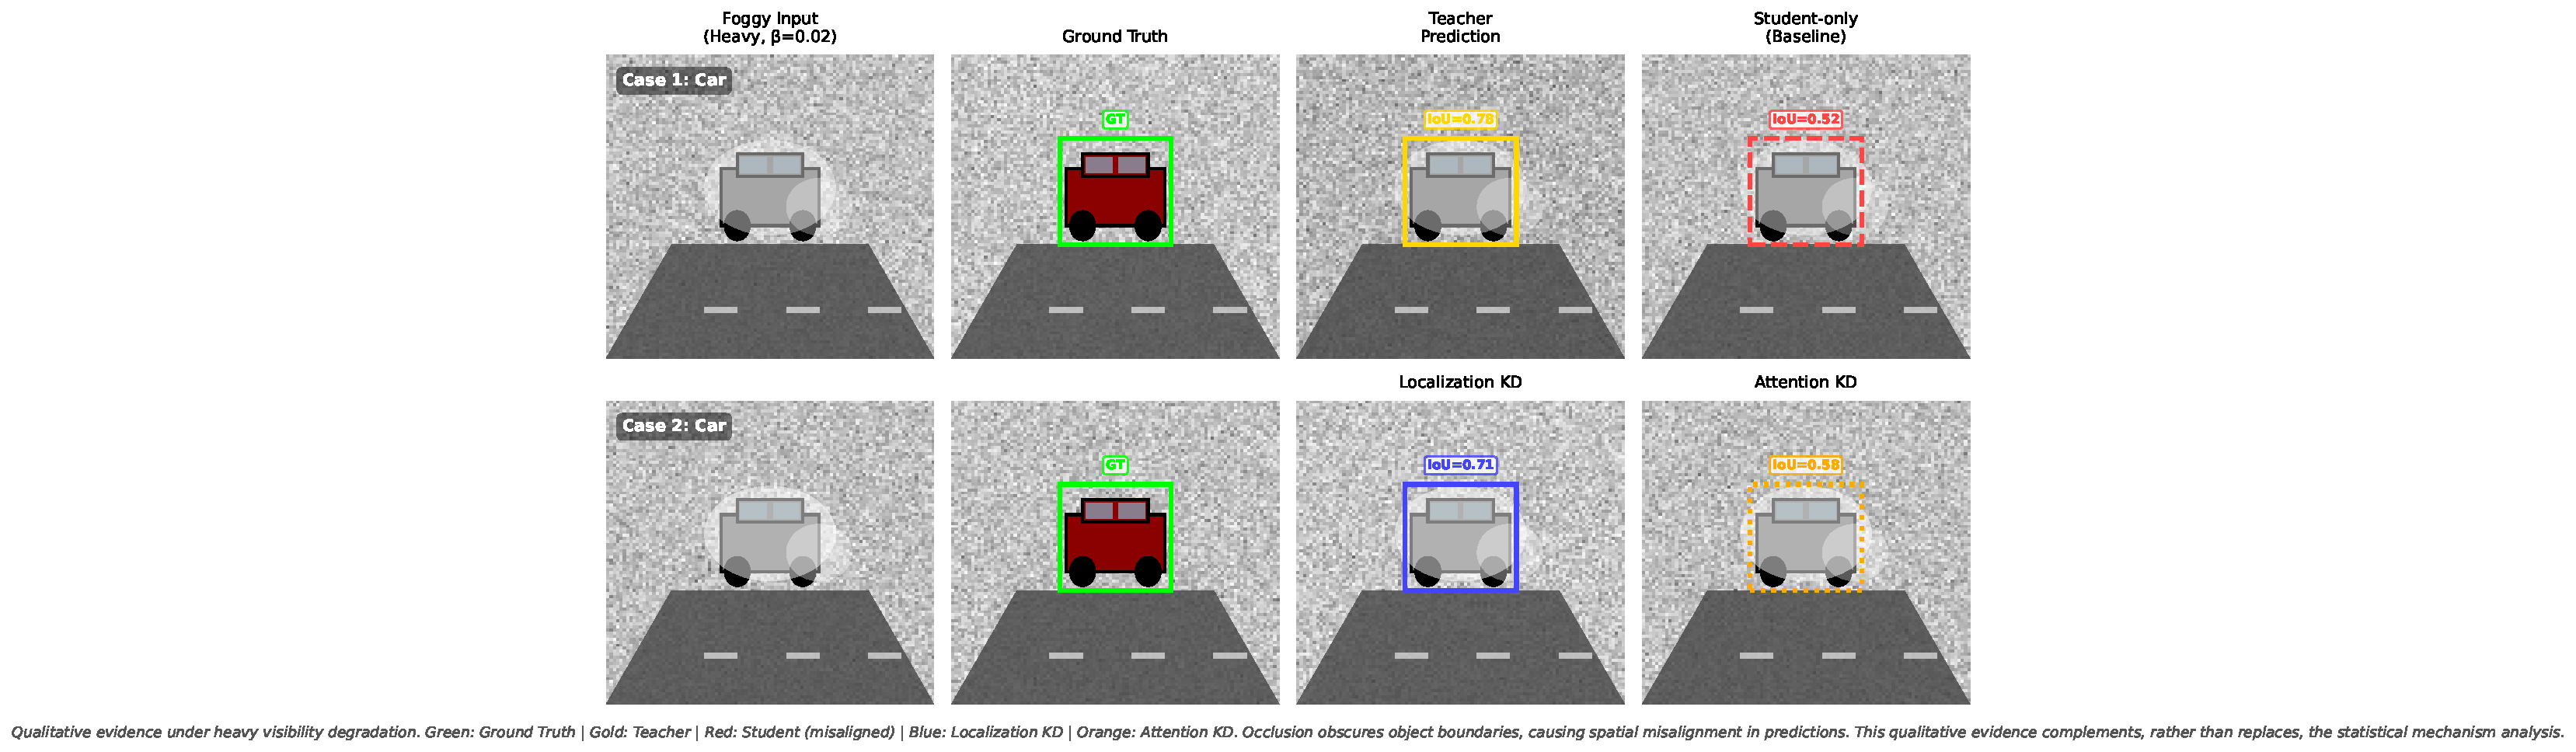
\includegraphics[width=0.95\textwidth]{figures/fig5_qualitative_occlusion.pdf}
\caption{Qualitative examples under heavy visibility degradation ($\beta=0.02$). Green boxes: Ground Truth; Gold: Teacher (IoU=0.78); Red (dashed): Student-only (IoU=0.52, spatially misaligned); Blue: Localization KD (IoU=0.71); Orange (dotted): Attention KD (IoU=0.58). Occlusion obscures object boundaries, causing spatial misalignment that is visually observable. This qualitative evidence complements, rather than replaces, the statistical mechanism analysis presented in \Cref{fig:mechanism_summary}.}
\label{fig:qualitative_occlusion}
\end{figure*}
